\subsubsection{Rotationsmatricer}
Hvis vi vil roterer et punkt eller en vektor omkring nul-punktet i et koordinatsystem kan vi bruge en rotationsmatrix\cite{rotationsmatricer}.
En rotationsmatrix er en matrix der, hvis ganget sammen med en anden matrix, roterer en vektor eller et punkt i et koordinatsystem.
\begin{align}\label{eu_eqn}
  R_x(\theta) = 
  \begin{bmatrix}
    1 & 0 & 0\\ 
    0 & cos \theta & - sin \theta\\ 
    0 & sin \theta & cos \theta
  \end{bmatrix}\\
    R_y(\theta) = 
  \begin{bmatrix}
    cos \theta  & 0 & sin \theta\\ 
    0           & 1 & 0\\ 
    -sin \theta & 0 & cos \theta
  \end{bmatrix}\\
    R_z(\theta) = 
  \begin{bmatrix}
    cos \theta & - sin \theta & 0\\ 
    sin \theta & cos \theta & 0\\
    0 & 0 & 1
  \end{bmatrix}
\end{align}
Indsætter vi mængden af radianer vi vil dreje vores vektor og ganger dem sammen, burde vektoren bliver drejet omkring nul-punktet med netop den mængde radianer.
For at sikre at vi har forstået brugen korrekt, vil vi nu forsøge at dreje en vektor i rummet omkring x-aksen ved hjælp af $R_x$. 
Vi har en vektor u:
\begin{equation}
  U=
  \begin{bmatrix}
    0 & 1 & 5
  \end{bmatrix}
\end{equation}
og rotationsvektor \begin{math}R_x\end{math}
\begin{equation}
  R_x(\theta) = 
  \begin{bmatrix}
    1 & 0 & 0\\ 
    0 & cos \theta & - sin \theta\\ 
    0 & sin \theta & cos \theta
  \end{bmatrix}
\end{equation}
Vi tager prik-produktet af dem, og indsætter 1 Radian i $R_x$:
\begin{align}
  0*0+1*0+5*0&=0\\
  0*0+1*cos(1)+5*sin(1)&=4.75\\
  0*0+1*(-sin(1))+5*cos(1)&=1.86
\end{align}
Og kalder det for vektor V og indsætter både U og V i Geogebra og får den til at udregne vinklen mellem dem:
\begin{figure}[H]
  \center
  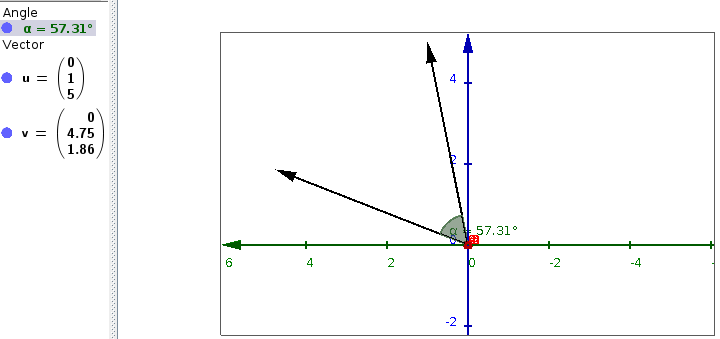
\includegraphics[width=12cm]{rotationsmatrix_eksempel.png}
  \caption{Eksempel på en rotationsmatrix}
  \label{fig:rotationsmatrix_eksempel}
\end{figure}
Geogebra udregner vinkler i grader, så vi omregner grader til radianer ved hjælp af ligningen:
\begin{equation}
  R=d/2*\pi/360=57,31/2*\pi/360\approx1
\end{equation}
Dette viser os at vektor $U$ blev drejet 1 radian, som forventet.
